\documentclass{sciposter}
\usepackage{lipsum}
\usepackage{epsfig}
\usepackage{amsmath}
\usepackage{amssymb}
\usepackage{multicol}
\usepackage{graphicx,url}
\usepackage[portuges, brazil]{babel}  
\usepackage[utf8]{inputenc}
\usepackage{listings}
\usepackage{color}
\usepackage{indentfirst}

\lstset{language=C++,
                basicstyle=\ttfamily,
                keywordstyle=\color{blue}\ttfamily,
                stringstyle=\color{red}\ttfamily,
                commentstyle=\color{green}\ttfamily,
                morecomment=[l][\color{magenta}]{\#}
}
%\usepackage{fancybullets}
\newtheorem{Def}{Definition}


\title{Mini Games com \\ Visão Computacional}
%Título do projeto

\author{Gabriel Vieira Figueiredo Tomaz, Tales Carlos de Pádua, Vinicius de Carvalho}

\institute
{Bacharelado em Ciência da Computação\\
Centro Universitário SENAC - Campus Santo Amaro
  (SENAC-SP)\\
  Av. Engenheiro Eusébio Stevaux, 823 -- Santo Amaro, São Paulo -- CEP 04696-000 -- SP -- Brasil}
%Nome e endereço da Instituição

\email{{ezefranca.br,colecionador.gabriel},{(@gmail.com})}
% Onde você coloca os emails dos integrantes


%\date is unused by the current \maketitle

\rightlogo[1]{respect_cube}
\leftlogo[1]{Senac-logo}
% Exibe os logos (direita e esquerda)
% Procure usar arquivos png ou jpg, e de preferencia mantenha na mesma pasta do .tex
%%%%%%%%%%%%%%%%%%%%%%%%%%%%%%%%%%%%%%%%%%%%%%%%%%%%%%%%%%%%%%%%%%%%%%%%%%%%%%%%
%%% Begin of Document

\begin{document}
%define conference poster is presented at (appears as footer)

\conference{{\bf BCC 15 anos}, 5º Projeto Integrador III - 15 anos do Bacharelado em Ciência da Computação, Senac, 06 de Junho de 2014, São Paulo, Brasil}

%\LEFTSIDEfootlogo 
% Uncomment to put footer logo on left side, and
% conference name on right side of footer

% Some examples of caption control (remove % to check result)

%\renewcommand{\algorithmname}{Algoritme} % for Dutch

%\renewcommand{\mastercapstartstyle}[1]{\textit{\textbf{#1}}}
%\renewcommand{\algcapstartstyle}[1]{\textsc{\textbf{#1}}}
%\renewcommand{\algcapbodystyle}{\bfseries}
%\renewcommand{\thealgorithm}{\Roman{algorithm}}

\maketitle

%%% Begin of Multicols-Enviroment
\begin{multicols}{3}

%%% Abstract
\begin{abstract}
O projeto consiste em 2 jogos controlados por algoritmos de visão computacional, sendo que um deles tem a base voltada para identificação de cores primárias e o outro uma rústica detecção de face por meio de bordas e padrões de rosto.
\end{abstract}

%%% Introduction
\section{Introducão}
Jogos interativos tem sido uma grande área a ser explorada à medida que a tecnologia e as formas de se produzir jogos avançam. A partir disso, aliando-se do que a visão computacional tem a oferecer como ferramenta para a interface entre o humano e o computador, tem-se que este trabalho soma esses conceitos para criar uma jogabilidade diferente baseada interamente em câmeras de vídeo, de modo que este novo meio de interação intensifique a experiência do usuário.

\newcommand{\imsize}{0.45\columnwidth}


\section{Objetivos}
Visando abordar uma maior quantidade de conhecimentos na área de visão computacional, o grupo tomou como estratégia a criação de dois jogos com interfaces diferentes, um baseado na detecção de cores e o outro baseado na detecção de faces.

Para o primeiro jogo, o principal objetivo era reconhecer com precisão 4 cores básicas: verde, amarelo, azul e vermelho. Com isto, foi possível estruturar o clássico jogo genius, que se basea em reconhecer estas cores descritas para validação de uma sequência correta de cores que o usuário deverá apresentar em frente à câmera.

O segundo jogo, um pouco mais complexo, envolve manipular as imagens vindas da câmera com o intuito de simplificar o que se está captando, sendo que, neste contexto, simplificar possibilita a detecção de certos padrões, como os de um rosto. Com o reconhecimento da face, o jogo se basea em um personagem dentro de um caminhão de sorvete utilizando o rosto para atender os pedidos de certos clientes.

\section{Metodologia}
No início do trabalho foi introduzido uma biblioteca, baseada em OpenCV, que faz a interface de acesso à câmera de maneira bem restrita, possibilitando apenas que houvesse contato com os quadros capturados da câmera fornecidos por uma matriz tridimensional onde a primeira dimensão é a altura (em pixels) da imagem, a segunda representa a largura (também em pixels) e a terceira são os componentes vermelho (red), verde (green) e azul (blue), respectivamente, do espaço de cores RGB. Todos os valores da matriz representam um número entre 0 e 255 do padrão RGB.

\subsubsection*{Jogo: Genius}

A principal ideia do reconhecimento das cores desse jogo foi o reconhecimento básico da cor vermelha, onde caso fosse verificado que o componente R da matriz fosse maior que a soma dos outros dois componentes, se tratava claramente da cor desejada. Apesar de funcionar relativamente bem para detecção de vermelho, as outras cores apresentavam uma resistência maior ao método devido a pequenas instabilidades e mudanças de luz, sendo necessário buscar algo mais sofisticado.
Após orientação e pesquisa surgiu a ideia de utilizar o espaço de cor HSV, onde H representa a cor propriamente dita, S a sua saturação e V o seu brilho. Com esta separação, ao contrário do que acontece no espaço RGB, pode-se facilmente determinar escopos (ranges) para cada cor, possibilitando assim uma filtragem mais precisa das cores desejadas.

A conversão do espaço de cor pode ser dada por:

\begin{figure}[ht]
\centering
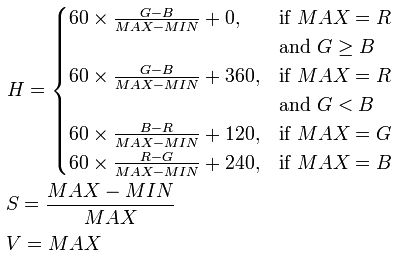
\includegraphics[width=8in]{img4.png}
\end{figure}


Um exemplo de resultado com a detecção da cor azul:

\begin{figure}[ht]
\centering
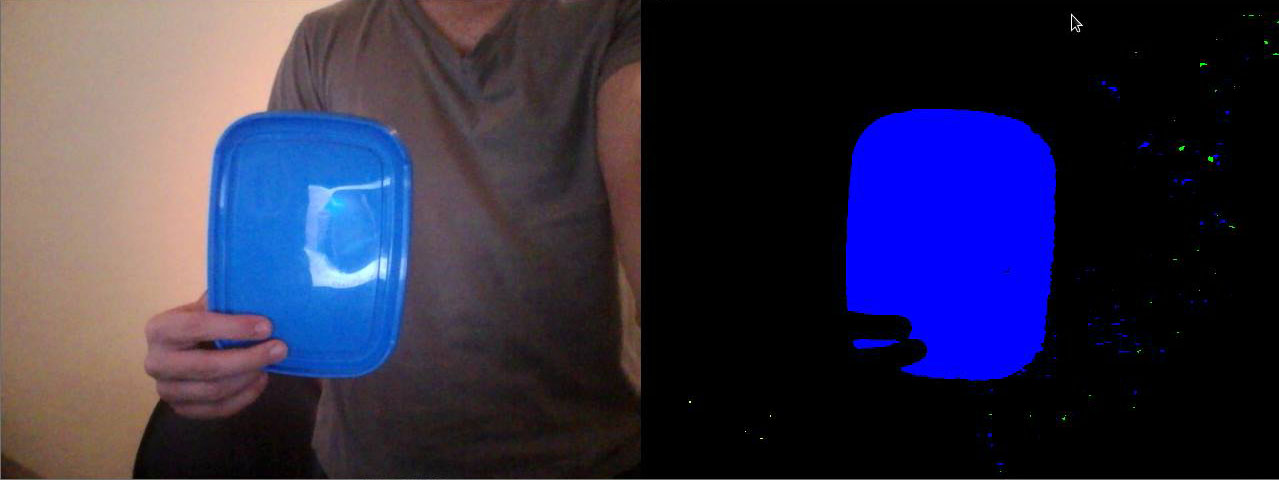
\includegraphics[width=8in]{img2.jpg}
\end{figure}

\subsubsection*{Jogo: Sorvete Hoje?}

A ideia deste jogo surgiu a partir do estudo de certos algoritmos que aliados permitem uma detecção bastante consistente de borda e, por consequência, uma boa detecção de face. Estudando formas de se detectar objetos de formato específico (como círculos, quadrados, etc) surgiu o principal algoritmo utilizado, o Filtro de Sobel, que será explicado mais adiante.

Aliado ao filtro, para que houvessem bordas mais consistentes, foi utilizado um algoritmo de binarização de imagem para delimitar bem. A técnica utilizada é conhecida como algoritmo de Otsu e também será descrita em um tópico seguinte.

Apenas o filtro, porém, não era suficiente para atingir os objetivos, visto que a manipulação de quadros da câmera pode ser um processo bastante custoso, o que gera uma experiência ruim para o usuário. Visando um modo de se otimizar este processo, antes de se aplicar o algoritmo do filtro foi utilizada uma conversão da imagem para escala de cinza, cujos benefícios serão descritos à seguir.

Por fim, para evitar impecilhos com a imagem de fundo da câmera, também foi agregado um algoritmo de remoção de fundo simples utilizando a fórmula matemática da Distância Euclidiana nos pixels dos quadros.

\subsubsection{Escala de Cinza}

O algoritmo de escala de cinza utilizado é bastante simples de ser aplicado no espaço de cor RGB, pois todos as cores obtidas ao se igualar os componentes R, G e B são tons de cinza. A fim de simplificar a quantidade de pixels que seriam processados, basta passar um algoritmo que soma as três componentes RGB de cada pixel, divide o valor por três e aplica o mesmo para as três componentes. \\

\begin{center}{A fórmula para o cálculo acima é dada por:}
$greyscale = \frac{R + G + B}{3}$ 
\end{center} \ \ 

Aplicando o valor de greyscale para as três componentes de cor, tem-se uma imagem descolorida cujos tons de cinza são aproximações das cores da imagem original. Com isso, pode-se aplicar os algoritmos seguintes com apenas um dos valores de R, G ou B e replicar o resultado nos demais, visto que são todos iguais, diminuindo assim a quantidade de processamento.

\subsubsection{Filtro de Sobel}

O Filtro de Sobel calcula o gradiente da intensidade da imagem em cada ponto, dando a direção da maior variação de claro para escuro e a quantidade de variação nessa direção por meio de duas matrizes quadradas de ordem 3, que são convoluídas com a imagem original para calcular aproximações das derivadas. Uma das matrizes representa a variação horizontal $Gx$ e a outra é a vertical $Gy$. \\

\begin{center}{Máscara de Sobel 3x3}
$$
Gx=\left[\begin{array}{rrr}
-1&0&+1\\
-2&0&+2 \\
-1&0&+1
\end{array}\right]\quad
Gy=\left[\begin{array}{ccc}
-1&-2&-1\\
0& 0& 0 \\
+1&+2&+1
\end{array}\right]
$$
\end{center}

E a partir disto, calcula-se a magnitude do gradiente:

$$
|G|=\sqrt{Gx^2 + Gy^2}
$$	

A variação de claro para escuro indica a presença de uma borda e com este gradiente aplicado nos canais RGB tem-se uma imagem composta apenas pelas bordas dos objetos que a compõem. Como a imagem utilizada está em escala de cinza, o resultado é uma imagem composta de bordas claras (próximas ao branco) com massas escuras (que tendem ao preto).

\subsubsection{Binarização da imagem}

Apesar dos diversos algoritmos para binarização de imagem, como os quadros que estão sendo trabalhados já estão bastante simplificados neste ponto, uma implementação baseada no algoritmo de Otsu é suficiente para atingir o objetivo de itensificar as bordas obtidas no Filtro de Sobel.

A ideia geral do método de Otsu é ter um valor limite onde se atribui a cor branca para os pixels que possuírem o canal RGB acima deste limite e preto para os que estiverem abaixo do mesmo. Essa limítrofe em geral é calculada a partir de fórmulas que utilizam a imagem para definir qual seria o valor mais adequado, entretanto, para a imagem com bordas, pode-se definir um valor constante e simplificar todo o processo.

\subsubsection{Remoção de fundo com Distância Euclidiana}

TODO TERMINAR AQUI

Quando se quer ignorar o fundo de um determinado cenário, pode-se aplicar a distância entre dois pontos definida por Euclides como <inserir a fórmula da distância euclidiana> comparando uma imagem que é composta apenas pelo fundo do cenário (que pode ser obtida a partir do primeiro quadro da câmera) com a imagem com que se deseja trabalhar (as demais imagens).
Este método é também bastante simples, porém resolve de maneira eficiente a intervenção de objetos no cenário que possam confundir os algoritmos citados a cima.

\subsubsection{Detecção de rosto}
O resultado de todos estes algoritmos alinhados é uma imagem de bordas bem definidas composta apenas pelo que não faz parte do cenário capturado pela câmera, ou seja, na grande parte dos casos haverá apenas a borda detalhada do jogador. \\

Exemplo de resultado dos algoritmos descritos:

INSERIR IMAGEM AQUI

À esquerda está a imagem original da câmera com exceção de uma pequena modificação no item 1, que é um retângulo vermelho indicando onde está a face do jogador. O item 2 representa a face do jogador em escala de cinza antes de ser aplicado o Filtro de Sobel, e o item 3 representa o mesmo após a aplicação do filtro e da binarização simples. O item 4 representa uma máscara que indica o local onde espera-se que o usuário posicione o rosto. Dentro das regiões coloridas compara-se a imagem tratada com valores esperados para um rosto humano (como muitos pixels brancos para os olhos e a boca, mas poucos para a face visto que não há muitas bordas na mesma).

\section{Resultados e Discussão}

Verificar os principais resultados obtidos de acordo com os objetivos propostos.\\

Genius :

Com a pesquisa e aplicação do metodo de conversao do espaço de cor conseguimos objeter grandes resultados com um algoritmo relativamente simples , e sem a aplicação de algum filtro 
o que nos forneceu uma detecção precisa de cores , para a realização deste jogo 
\begin{itemize}
\item Set all elements of array {\tt S} to zero
\item For all $x \in X$ increment {\tt S}[$\Omega_X(x)$] by one.
\end{itemize}

To compute the pattern \emph{moment} spectrum, the only thing that needs to be
changed is the way {\tt S}[$\Omega_X(x)$] is incremented. As shown in Algorithm
\ref{alg:spect}.

\begin{algorithm}
\begin{itemize}
\item Set all elements of array {\tt S} to zero
\item For all $(x,y) \in X$ increment {\tt S}[$\Omega_X(x,y)$] by
$x^iy^j$.
\end{itemize}
\caption{ Algorithm for computation of pattern moment
spectrum of order $ij$. \label{alg:spect}}
\end{algorithm}

This algorithm can
readily be adapted to other granulometries, simply by computing the
appropriate opening transform.

\begin{figure}
\begin{center}
\begin{tabular}{c c}

\end{tabular}
\end{center}
\caption{ \label{fig:tauspect}
The opening transform using city-block metric: (a) opening transform of
Fig. 1(c); (b) pattern spectrum; (c) pattern variance-$x$;
(d) variance-$y$ spectra.}
\end{figure}


\renewcommand{\imsize}{0.3\columnwidth}
\begin{figure}
\begin{center}
\end{center}
\caption{ \label{fig:binspect} Pattern mean-$x$ (top) and variance-$x$
(bottom) spectra: the three collumns show spectra for Fig. 1(a), (b) and (c)
from left to right respectively.  Unlike the standard pattern spectra,
these spatial pattern spectra can distinguish the three images.}
\end{figure}

\section{Conclusão}

Sitting on a corner all alone,
staring from the bottom of his soul,
watching the night come in from the window
\\
It'll all collapse tonight, the fullmoon is here again
In sickness and in health, understanding so demanding
It has no name, there's one for every season
Makes him insane to know
\\
 
%%% References

%% Note: use of BibTeX als works!!

\bibliographystyle{plain}
\begin{thebibliography}{1}

%\bibitem{Flusser:Suk:93}
%J.~Flusser and T.~Suk.
%\newblock Pattern recognition by affine moment invariants.
%\newblock {\em Pattern Recognition}, 26:167--174, 1993.

%\bibitem{Hu:62}
%M.~K. Hu.
%\newblock Visual pattern recognition by moment invariants.
%\newblock {\em IRE Transactions on Information Theory}, IT-8:179--187, 1962.

%\bibitem{maragos89:_patter}
%P.~Maragos.
%\newblock Pattern spectrum and multiscale shape representation.
%\newblock {\em IEEE Trans. Patt. Anal. Mach. Intell.}, 11:701--715, 1989.

%\bibitem{Meijster:Wilkinson:PAMI}
%A.~Meijster and M.~H.~F. Wilkinson.
%\newblock A comparison of algorithms for connected set openings and closings.
%\newblock {\em IEEE Trans. Patt. Anal. Mach. Intell.}, 24(4):484--494, 2002.

%\bibitem{Nacken:thesis}
%P.~F.~M. Nacken.
%\newblock {\em Image Analysis Methods Based on Hierarchies of Graphs and
%  Multi-Scale Mathematical Morphology}.
%\newblock PhD thesis, University of Amsterdam, Amsterdam, The Netherlands,
%  1994.
  
%referencia do sobel
\bibitem{Sobel1968}
{SOBEL, Irvin}
\newblock A 3x3 isotropic gradient operator for image processing.
\newblock Never published but presented at a talk at the Stanford Artificial
  Project, 1968.
\end{thebibliography}

\end{multicols}

\end{document}